% !TEX TS-program = XeLaTeX
\documentclass[11pt, twoside]{imsproc}
\usepackage{graphicx}
\usepackage{geometry}
\usepackage{amsmath,amsthm,amssymb,graphicx,tikz,fancyhdr} 
\usepackage{booktabs}
\usepackage[colorlinks,citecolor=blue]{hyperref}
\setcounter{page}{1}
\newtheorem{de}{تعریف}[section]
\newtheorem{exa}[de]{مثال}
\newtheorem{alg}[de]{الگوریتم}
\newtheorem{lemma}[de]{لم}
\newtheorem{theorem}[de]{قضیه}
\newtheorem{corollary}[de]{نتیجه}
\newtheorem{example}[de]{مثال}
\newtheorem{remark}[de]{تبصره}
\newtheorem{problem}[de]{مسأله}
\newtheorem{proposition}[de]{گزاره}
\geometry{left=2.5cm,right=2.5cm,top=3cm,bottom=3cm,headsep=1.1cm}
\footskip 0.7cm
%------------------------------------------------------------------------------------%
\newcommand*{\publname}{%
\begin{tabular}{c}

\includegraphics[width=1.8cm]{UI-Logo.jpg}\\
\url{http://www.ui.ac.ir}
\vspace{0.2cm}
\end{tabular}
\hfill
\begin{tabular}{c}\toprule
\vspace{0.1cm}
\scriptsize \bfseries ریاضی و جامعه\\
\vspace{0.1cm}
\scriptsize
شاپا (چاپی): 2345-6493، شاپا(الکترونیکی): 2345-6507 \\
\vspace{0.1cm}
\scriptsize
جلد x، شماره x (1400)، صص. xx-xx\\
\scriptsize
\copyright{} 1xxx دانشگاه اصفهان \\ \bottomrule
\end{tabular}
\hfill
\begin{tabular}{c}

\includegraphics[width=2.2cm]{JMS-Logo.jpg}\\
\url{http://math-sci.ui.ac.ir}
\vspace{-0.2cm}
\end{tabular}
}
%------------------------------------------------------------------------------------%
\usepackage[para*]{manyfoot}
\SetFootnoteHook{\setLTR}
\DeclareNewFootnote[para]{A}
\usepackage{xepersian}
\makeatletter
\let\c@footnoteA\c@footnote
\makeatother
\let\LTRfootnote\footnoteA
\AtBeginDocument{\label{firstpage}}
\AtEndDocument{\label{lastpage}}
\settextfont[Scale=1.1]{XB Niloofar}
\setlatintextfont [Scale=0.9]{Times New Roman}
\linespread{1.35}
\newsavebox\uilogo
\newsavebox\nologo
\sbox\uilogo{
\includegraphics[width=0.8cm]{UI-Logo.pdf}}
\sbox\nologo{
\includegraphics[width=1cm]{JMS-Logo.jpg}}
\makeatletter
\def\seriesno#1{\gdef\@seriesno{#1}}
\def\issueno#1{\gdef\@issueno{#1}}
\def\publicationname#1{\gdef\@publicationname{#1}}
\def\ps@ijheadings{\ps@empty
  \def\@evenhead{%
   \parbox{\textwidth}{%
    \setTrue{runhead}%
    \normalfont\scriptsize
    \usebox\uilogo\hfill
    \def\thanks{\protect\thanks@warning}%
  \leftmark{}{}, \@publicationname/
    جلد x،
   % \@seriesno{}
    شماره x 
   % \@issueno
 (1xxx) \pageref{firstpage}--\pageref{lastpage}
    \hfill
   \usebox\nologo\vskip0pt
     \vskip-7pt
     \rule{\textwidth}{0.5pt}
      \vskip-12pt
        \rule{\textwidth}{0.5pt}
    }}
  \def\@oddhead{%
   \parbox{\textwidth}{%
    \setTrue{runhead}%
    \normalfont\scriptsize
    \usebox\uilogo\hfill
    \def\thanks{\protect\thanks@warning}%
    \rightmark{}{}, \@publicationname/
    جلد x،
    %\@seriesno{}
    شماره x 
    %\@issueno
 (1xxx) \pageref{firstpage}--\pageref{lastpage}
    \hfill
   \usebox\nologo\vskip0pt
     \vskip-6pt
     \rule{\textwidth}{0.5pt}
      \vskip-12pt
        \rule{\textwidth}{0.5pt}
    }}
   \def\@evenfoot{\normalfont\small\thepage
     \hfill \scriptsize{\url{http://dx.doi.org/10.22108/MSCI.xxxx}}\hfill}
    \def\@oddfoot{\normalfont\small\hfill\scriptsize{\url{http://dx.doi.org/10.22108/MSCI.xxxx}}\hfill\thepage}
 }%   
\def\enddoc@text{%
\ifx\@empty\@translators \else\@settranslators\fi
  \ifx\@empty\addresses \else\@setaddresses\fi}
  
\renewcommand*{\@makefnmark}{\hbox{\@textsuperscript{\normalfont\@thefnmark}}}
  \def\MFL@fnotepara#1#2#3{\let\@thefnmark\@empty
    \NCC@makefnmark{\latinfont #2}%
    \MFL@insert#1{\reset@font\footnotesize
      \ifx\@thefnmark\@empty \@tempswafalse \else
        \@tempswatrue
        \protected@edef\@currentlabel{\@thefnmark}%
      \fi
      \color@begingroup
        \if@tempswa
          \setbox\@tempboxa\hbox{\@makefnmark}%
          \ifMFL@paraindent
            \@tempdima.8em \advance\@tempdima-\wd\@tempboxa
            \ifdim \@tempdima<\z@ \@tempdima\z@ \fi
          \else
            \@tempdima\z@
          \fi
        \fi
        \setbox\@tempboxa\hbox{%
          \if@tempswa
            \hskip\@tempdima\unhbox\@tempboxa\nobreak
          \fi
          \ignorespaces\resetlatinfont#3\unskip\strut
          \ifMFL@split \penalty\m@ne\space \else
            \penalty-10 \hskip\footglue
          \fi
        }%
        \dp\@tempboxa\z@ \ht\@tempboxa\MFL@fudgefactor\wd\@tempboxa
        \box\@tempboxa
      \color@endgroup
    }%
  }
\long\def\@footnotetext#1{\insert\footins{%
   \if@RTL@footnote\@RTLtrue\else\@RTLfalse\fi%
    \reset@font\tiny
    \interlinepenalty\interfootnotelinepenalty
    \splittopskip\footnotesep
    \splitmaxdepth \dp\strutbox \floatingpenalty \@MM
    \hsize\columnwidth \@parboxrestore
    \protected@edef\@currentlabel{%
       \csname p@footnote\endcsname\@thefnmark
    }%
    \color@begingroup
      \@makefntext{%
        \rule\z@\footnotesep\ignorespaces\if@RTL@footnote#1\else\latinfont#1\fi\@finalstrut\strutbox}%
    \color@endgroup}}%
%\footdir@temp\footdir@my@ORG@xepersian@footnotetext\@footnotetext{\bidi@footdir@footnote}%
\makeatother
\pagestyle{ijheadings}
\seriesno{1}
\issueno{1}
\publicationname{نشریه ریاضی و جامعه}
\title{عنوان مقاله}
\author[نویسنده اول و نویسنده دوم ، مترجم ]
{ نویسنده اول و $^*$ نویسنده دوم\\
اگر مقاله به زبان دیگری باشد در اینجا نام مترجم آورده شود}

\thanks{
عبارات و کلمات کليدي: {کلمات کلیدی آورده شود.}\\
دبیرتخصصی رابط: -------------\\  
نوع مقاله: ----------------\\
تاریخ دریافت: 1400/xx/xx
\quad
تاریخ پذیرش: 1400/xx/xx 
\newline
\url{http://dx.doi.org/10.22108/MSCI.xxxx}
}
\copyrightinfo{}{(دانشگاه اصفهان)}
%\subjclass[2010]{Analysis; topology}
\makeatletter
\def\ps@firstpage{\ps@plain
\def\@oddfoot{\normalfont\small\hfil\thepage\hfil
\global\topskip\normaltopskip}%
\let\@evenfoot\@oddfoot
\def\@oddhead{\@serieslogo\hss}%
\let\@evenhead\@oddhead % in case an article starts on a left-hand page
}
%%%%%%%%%%%%%%%%%
\settextfont[Scale=1.1]{XB Yas}
%%%%%%%%%%%%%%%%%%%%%%%
\makeatother
\begin{document}
\begin{abstract}
در این قسمت چکیده مقاله نوشته می شود.
\end{abstract}
\maketitle
\section{مقدمه}

دراین قسمت مقدمه  نوشته می شود.
\section{متن اصلی}
\vskip 0.4 true cm
در این قسمت متن اصلی نوشته می شود. در زیر یک متن نمونه نوشته شده است.\\
در شیوه‌ی پیشنهادی برای وضوح برتر توسط نگارندگان ، هر یک از تصاویر باوضوح بالا، به عنوان تصویر آموزشی، متناظر با قسمتی از تصویرِ باوضوح پایین هستند.  تصاویر آموزشی می‌توانند تفاوتهایی با تصویر اصلی از نقطه نظر شدت روشنائی یا زاویه‌ی اخذ داشته باشند. 
 این تفاوتها می‌تواند ناشی از برداشت عکسها \footnote{یک زیر نویس پارسی}در زمانهای متفاوت و یا با دوربینهای متفاوت و از زوایای مختلف باشد. در این شیوه ابتدا تصویر با وضوح پایین به اندازه‌ی مطلوب بزرگ شده و سپس  تبدیل مناسبی برای نگاشت هر یک از تصاویر آموزشی بر روی تصویر مورد نظر با استفاده از  نقاط کلیدی \lr{SIFT}\LTRfootnote{ Scale Invariant Feature Transform (SIFT)} و الگوریتم \lr{RANSAC}\LTRfootnote{ RANdom SAmple Consensus (RANSAC)} در قالب ماتریس هوموگرافی\LTRfootnote{ Homography matrix} پیدا می‌شود. 

\subsection{الگوریتم لوکاس-کاناد}
 هدف در شیوه‌ی ثبت تصویر لوکاس-کاناد کمینه‌سازی مجموع مربع تفاضلات زیر بین تصویر آموزشیِ $T(\mathbf{x})$ و نگاشت تصویر ورودیِ $I(\mathbf{x})$ است:
 \begin{equation}
\label{eq:SSD_L2Norm}
    SSD=\sum_x[m-T(\mathbf{x})]^2
\end{equation}
که در آن $m$ بیانگر مدل تبدیل‌ (در اینجا پروجکتیو)، $\mathbf{p}=(p_1,\dots,p_8)^T$ پارامترهای مدل تبدیل، $m$ نگاشت تصویر ورودی $I$ بر روی مختصات تصویر آموزشی $T$ و $\mathbf{x} =(x,y)^T$ مختصات یک پیکسل می‌باشد.
 کمینه‌سازی \eqref{eq:SSD_L2Norm} نسبت به $\mathbf{p}$ انجام می‌شود. 
در شیوه‌ی لوکاس-کاناد فرض بر آن است که در ابتدا تخمینی از مدل دردست بوده و در یک فرآیند تکراری این تخمین بهبود داده می‌شود؛
در هر دور ابتدا عبارت زیر بر اساس $\triangle\mathbf{p}$ کمینه شده:
\begin{equation}
\label{eq:SSD_L2Norm_deltap}
    \sum_x[I(\mathbf{W}(\mathbf{x;\mathbf{p+\triangle p}}))-T(\mathbf{x})]^2
\end{equation}
 و سپس پارامترها بروزرسانی می‌شوند:
\begin{equation}
    \mathbf{p}\leftarrow\mathbf{p+\triangle p}
\end{equation}
دو مرحله‌ی فوق تا مادامیکه الگوریتم همگرا نشده است تکرار خواهند شد. در فرآیند کمینه‌سازی، $\mathbf{\triangle p}$ به صورت زیر محاسبه می‌شود:
\begin{equation}
\label{eq:deltap}
    \triangle\mathbf{p} = H^{-1} \sum_x[\nabla I{W}{p}]^T[T(\mathbf{x})-m]
\end{equation}
که در آن $H$، ماتریس هسین تقریبی\LTRfootnote{ Approximate Hessian Matrix}، به صورت زیر بدست می‌آید:
\begin{equation}
\label{eq:Hessian}
  H = \sum_x[\nabla I{W}{p}]^T[\nabla I{W}{p}]
\end{equation}

\section{جدول‌ها}
\vskip 0.4 true cm
هر جدول بايد دارای شماره و عنوان (توضيح) باشد، كه به صورت وسط چين در بالاي جدول  شماره‌گذاری می شود. بهتر است جدول‌ها در داخل متن و پس از جايی كه به آنها ارجاع مي‌شود، درج گردند.  هر جدول با يك سطر خالی فاصله از متن ماقبل و مابعد آن قرار گيرد. يك نمونه جدول مطابق دستورالعمل در زير آمده است: (توجه شود كه خود جدول نيز بايد در موقعيت وسط چين نسبت به طرفين كاغذ قرار گيرد).
\\

\begin{center}
\par
\begingroup%
  \makeatletter
  \def\@captype{table}%
  \makeatother
  \caption{جدول نمونه }%
\endgroup%
\begin{tabular}{|c|p{2in}|} 
\hline عنوان & توضیحات \\ 
\hline  &  \\ 
\hline  &  \\ 
\hline  &  \\ 
\hline 
\end{tabular} 
\end{center}
\section{شكل‌ها و نمودارها}
\vskip 0.4 true cm
هر شكل و نمودار بايد دارای شماره و عنوان (توضيح) باشد كه به صورت وسط چين در زير آن با قلم پررنگ  و به ترتيب از 1 شماره‌گذاری می شود. شكل ‌ها در داخل متن و در جايی كه به آنها ارجاع می شود، درج گردند. ذكر واحد كميت‌ها در شكل‌ها الزامی است. در تهيه شكل‌ها توجه كنيد كه اندازه اعداد، واژه‌ها، كميت‌ها و راهنمای منح هر شكل را با يك سطر خالی فاصله از متن ماقبل و مابعد آن قرار دهيد. (توجه شود كه خود شكل ها و نمودارها نيز، همانند جدول ها بايد در موقعيت وسط چين نسبت به طرفين كاغذ قرار گيرند.)
\\
\begin{figure}[ht]
\centering
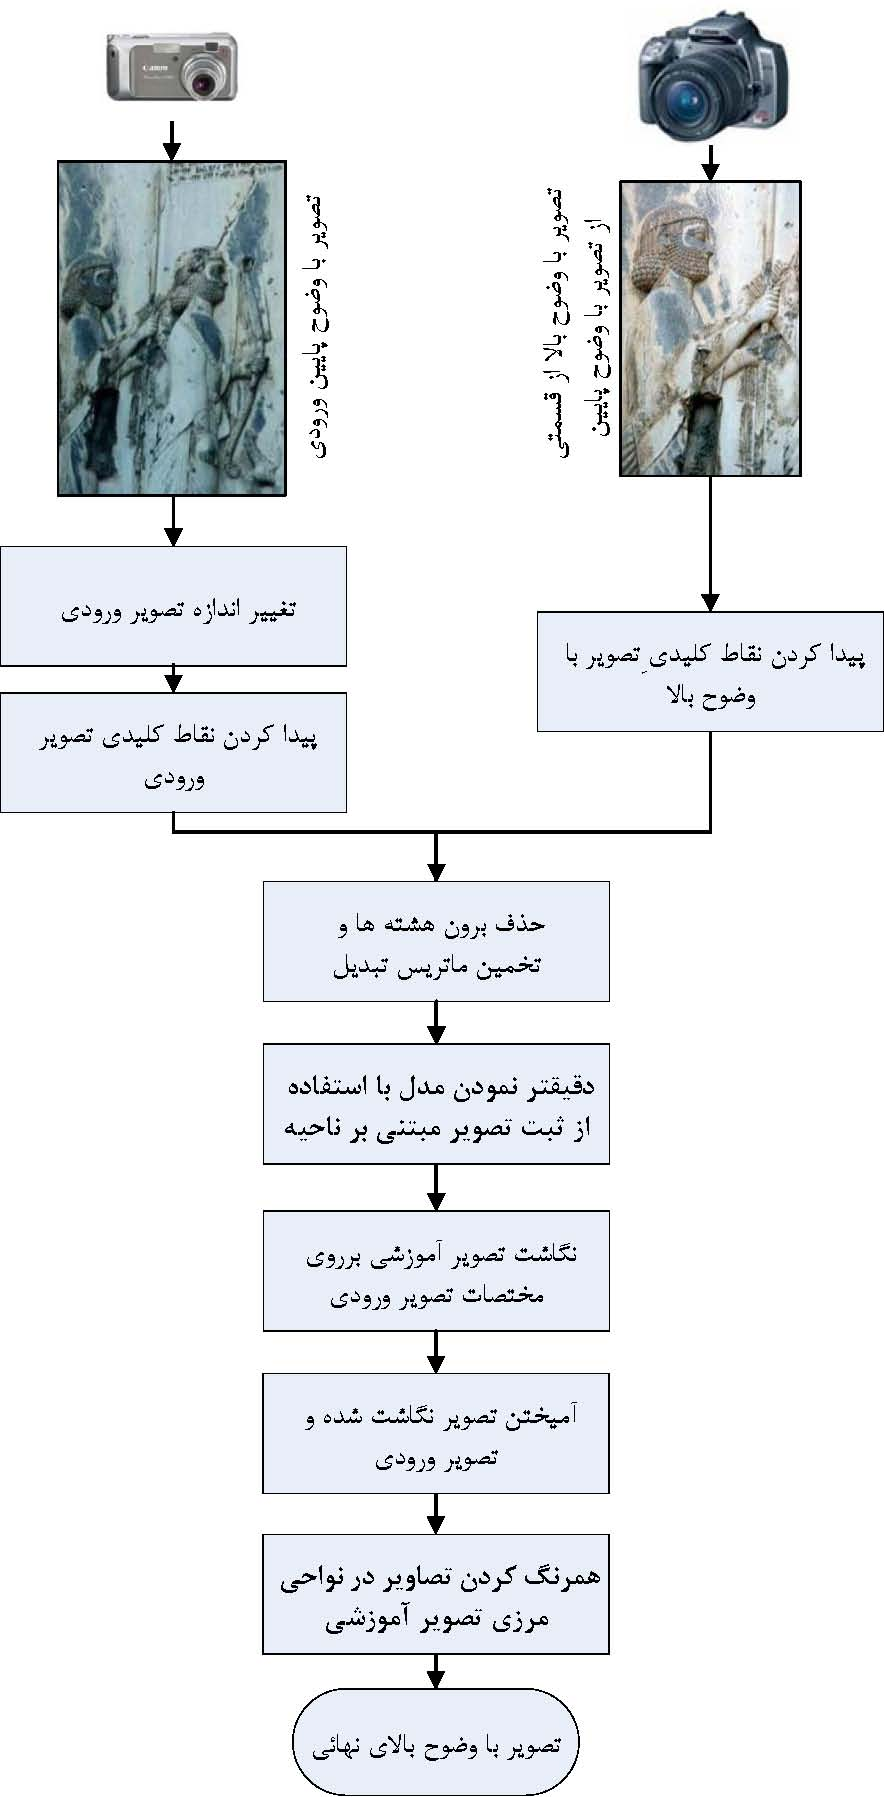
\includegraphics[width=55mm]{Fig-1} 
\caption{\label{shir}\small نمونه شكل }
\end{figure}

\subsection{نتایج مقایسه‌ای ثبت تصویر}

شکل \ref{fig:RMS} میانگین مربعات خطا را در هر دور از الگوریتم‌های 1و2 برای سه روش فوق‌الذکر در یک اجرای نمونه نشان می‌دهد. روش پیشنهادی با \lr{LKSSIM-LM} مشخص شده است. حداکثر تعداد تکرار 15 درنظر گرفته شده بوده است. همانگونه که دیده می‌شود روش پیشنهادی از همگرائی سریعتری نسبت به هر دو شیوه‌ی دیگر برخوردار است. 

شکل \ref{fig:Conv_Iter} میانگین تعداد تکرارها تا همگرا شدن را برای هر سه روش فوق و در مقادیر مختلف نویز نشان می‌دهد. در هیچ یک از آزمایشات روی این تصاویر، روش \lr{LK} واگرا نشده بود.
\eject

\begin{figure}[ht]
\centering 
\includegraphics*[height=40mm,width = 0.4\columnwidth]{Fig-2}
\caption{ \small اسم نمودار 1. }
\label{fig:RMS}
\end{figure}

\begin{figure}[ht]
\centering
\includegraphics*[height=30mm, width = 0.3\columnwidth]{Fig-3}
\caption{ \small اسم نمودار 2.}
\label{fig:Conv_Iter}
\end{figure}
%\section{تشكر وقدردانی}
%\vskip 0.4 true cm
%در این قسمت تشکر و قدردانی آورده می شود.\\%
%\vskip 0.4 true cm

\begin{thebibliography}{99}%
\begin{LTRbibitems}
\resetlatinfont

\bibitem{Baillie}
R. Baillie, Long memory processes and fractional integration in econometrics, \emph{J.  Econometrics},  \textbf{73}  (1996) 5–59.
\bibitem{Pishkoo2}
N. Delfan, A. Pishkoo, M.  Azhini and M. Darus, Using fractal calculus to express electric potential and electric field in terms of staircase and characteristic functions, \emph{Eur. J.  Pure   Appl.  Math.}, \textbf{13} (2020) 19-32.
\bibitem{Falconer}
K. Falconer, \emph{Techniques in Fractal Geometry}, Wiley,  New York, 1997.
\bibitem{Haynes}
C. P. Haynes and A. D.  Roberts, Generalization of the fractal Einstein law relating conduction and diffusion on networks, \emph{Phys. Rev.  Lett.}, \textbf{103} (2009) 020601. doi: 10.1103/PhysRevLett.103.020601.
\bibitem{Satin2}
S. Satin and  A. D. Gangal, Langevin equation on fractal curves, \emph{Fractals}, \textbf{24} (2016) 1650028, 7 pp.  doi: 10.1142/s0218348x16500286.
\end{LTRbibitems}

\bibitem{2}
م. ح. اکرمی، حسابان کسری از نظریه تا کاربرد،
\emph{ریاضی و جامعه}،
 \textbf{4} (1396) 56-69.

\bibitem{2}
س. یاسمی، م. پورنکی، {\em مقدمه‌ای بر نظریه‌ی مدول‌ها}، مؤسسه‌ی انتشارات علمی دانشگاه صنعتی شریف، 
   ۱۳۸۴.
\end{thebibliography}
%------------------------------------------------------------------------------------------------
%نوشتن بیوگرافی نویسندگان الزامی می باشد.

\bigskip
\bigskip 

\noindent \rule{.4\linewidth}{0.8pt}\\
\noindent\footnotesize{\bfseries نام و نام خانوادگی نویسنده اول (اگرمقاله به زبان دیگری باشد نام و نام خانوادگی مترجم) } \\
\footnotesize{اصفهان، خيابان هزار جريب، دانشگاه اصفهان، گروه ریاضی } \\
abc@yahoo.com\\\\
\begin{tabular}{p{2 cm} p{14 cm} }

\includegraphics[width=20mm]{Image1} 
&\vspace{-1.5cm}
\footnotesize

نویسنده اول (یا مترجم) متولد مهرماه ماه 1361 در شهر اصفهان است. وی در سال 1380 وارد مقطع كارشناسی رشته رياضی محض دانشگاه اصفهان شد و در سال 1385 وارد مقطع كارشناسی ارشد رشته رياضی محض شد.\\
\end{tabular}\\\\
\noindent\footnotesize{\bfseries نام و نام خانوادگی نویسنده دوم } \\
\footnotesize{تهران، دانشگاه تهران، گروه ریاضی } \\
 def@gmail.com\\\\
\begin{tabular}{p{2 cm} p{14 cm} }

\includegraphics[width=20mm]{Image2} 
&\vspace{-1.5cm}
\footnotesize

نویسنده دوم متولد مرداد ماه 1368 در شهر تهران است. وی در سال 1386 وارد مقطع كارشناسی رشته رياضی كاربردی دانشگاه تهران شد و در سال 1390  وارد مقطع كارشناسی ارشد رشته رياضی كاربردی شد.
\end{tabular}
\end{document}